\documentclass[12pt]{article}
\PassOptionsToPackage{table,x11names,dvipsnames,rgb}{xcolor}

\usepackage[utf8]{inputenc}
\usepackage[british]{babel}

\usepackage{xstring}

\usepackage{tikz}
\usetikzlibrary{arrows,shapes,automata,positioning,trees,shadows,mindmap,decorations}
%% From <http://tex.stackexchange.com/questions/137357/how-to-draw-an-arrow-with-two-colors>
%% <http://tex.stackexchange.com/a/137438>
\usetikzlibrary{fadings,decorations.pathmorphing}

\makeatletter
\newif\iftikz@shading@path

\tikzset{
    % There are three circumstances in which the fading sep is needed:
    % 1. Arrows which do not update the bounding box (which is most of them).
    % 2. Line caps/joins and mitres that extend outside the natural bounding 
    %    box of the path (these are not calculated by PGF).
    % 3. Other reasons that haven't been anticipated.
    shading xsep/.store in=\tikz@pathshadingxsep,
    shading ysep/.store in=\tikz@pathshadingysep,
    shading sep/.style={shading xsep=#1, shading ysep=#1},
    shading sep=0.0cm,
}

\def\tikz@shadepath#1{% 
    % \tikz@addmode installs the `modes' (e.g., fill, draw, shade) 
    % to be applied to the path. It isn't usualy for doing more
    % changes to the path's construction.
    \iftikz@shading@path%
    \else%
        \tikz@shading@pathtrue%
        % Get the current path.
        \pgfgetpath\tikz@currentshadingpath%
        % Get the shading sep without setting any other keys.
        \begingroup%
            \pgfsys@beginscope% <- may not be necessary
            \tikzset{#1}%
            \xdef\tikz@tmp{\noexpand\def\noexpand\tikz@pathshadingxsep{\tikz@pathshadingxsep}%
                \noexpand\def\noexpand\tikz@pathshadingysep{\tikz@pathshadingysep}}%
            \pgfsys@endscope%
        \endgroup
        \tikz@tmp%
        % Get the boudning box of the current path size including the shading sep
        \pgfextract@process\pgf@shadingpath@southwest{\pgfpointadd{\pgfqpoint{\pgf@pathminx}{\pgf@pathminy}}%
            {\pgfpoint{-\tikz@pathshadingxsep}{-\tikz@pathshadingysep}}}%%
        \pgfextract@process\pgf@shadingpath@northeast{\pgfpointadd{\pgfqpoint{\pgf@pathmaxx}{\pgf@pathmaxy}}%
            {\pgfpoint{\tikz@pathshadingxsep}{\tikz@pathshadingysep}}}%
        % Clear the path
        \pgfsetpath\pgfutil@empty%                          
        % Save the current drawing mode and options.
        \let\tikz@options@saved=\tikz@options%
        \let\tikz@mode@saved=\tikz@mode%
        \let\tikz@options=\pgfutil@empty%
        \let\tikz@mode=\pgfutil@empty%
        % \tikz@options are processed later on.
        \tikz@addoption{%
            \pgfinterruptpath%
            \pgfinterruptpicture%
                \begin{tikzfadingfrompicture}[name=.]
                \pgfscope%
                    \tikzset{shade path/.style=}% Make absolutely sure shade path is not inherited.
                    \path \pgfextra{%
                        % Set the softpath. Any transformations,draw=none} in #1 will have no effect.
                        % This will *not* update the bounding box...
                        \pgfsetpath\tikz@currentshadingpath%
                        % ...so it is done manually.
                        \pgf@shadingpath@southwest
                        \expandafter\pgf@protocolsizes{\the\pgf@x}{\the\pgf@y}%
                        \pgf@shadingpath@northeast%
                        \expandafter\pgf@protocolsizes{\the\pgf@x}{\the\pgf@y}%
                        % Install the drawing modes and options.
                        \let\tikz@options=\tikz@options@saved%
                        \let\tikz@mode=\tikz@mode@saved%
                    };
                    % Now get the bounding box of the picture.
                    \xdef\pgf@shadingboundingbox@southwest{\noexpand\pgfqpoint{\the\pgf@picminx}{\the\pgf@picminy}}%
                    \xdef\pgf@shadingboundingbox@northeast{\noexpand\pgfqpoint{\the\pgf@picmaxx}{\the\pgf@picmaxy}}%
                    \endpgfscope
                \end{tikzfadingfrompicture}%
            \endpgfinterruptpicture%
            \endpgfinterruptpath%
            % Install a rectangle that covers the shaded/faded path picture.
            \pgftransformreset%
            \pgfpathrectanglecorners{\pgf@shadingboundingbox@southwest}{\pgf@shadingboundingbox@northeast}%
            %
            % Reset all modes.
            \let\tikz@path@picture=\pgfutil@empty%
            \tikz@mode@fillfalse%
            \tikz@mode@drawfalse%
            \tikz@mode@tipsfalse%
            \tikz@mode@doublefalse%
            \tikz@mode@clipfalse%
            \tikz@mode@boundaryfalse%
            \tikz@mode@fade@pathfalse%
            \tikz@mode@fade@scopefalse%
            % Now install shading options.
            \tikzset{#1}%
            \tikz@mode%
            % Make the fading happen.
            \def\tikz@path@fading{.}%
            \tikz@mode@fade@pathtrue%
            \tikz@fade@adjustfalse%
            % Shift the fading to the mid point of the rectangle
            \pgfpointscale{0.5}{\pgfpointadd{\pgf@shadingboundingbox@southwest}{\pgf@shadingboundingbox@northeast}}%
            \edef\tikz@fade@transform{shift={(\the\pgf@x,\the\pgf@y)}}%
            \pgfsetfading{\tikz@path@fading}{\tikz@do@fade@transform}%
            \tikz@mode@fade@pathfalse%              
        }%
    \fi%
}
\tikzset{
    shade path/.code={%
        \tikz@addmode{\tikz@shadepath{#1}}%
    }
}

% requires tikz
\usepackage{colortbl}

\usepackage{float}
\usepackage{graphicx}
\usepackage[normalem]{ulem}

%% use as
%%     \vertcenterimage{\includegraphics{*}}
\newcommand{\vertcenterimage}[1]{\raisebox{-.5\height}{#1}}

%% use as
%%     \flipbox{\includegraphics{*}}
\newcommand{\flipbox}[1]{\scalebox{1}[-1]{#1}}

\usepackage{amsmath}
\usepackage{amsfonts}
\usepackage{bm} % bold mathematics (\bm command)

% set-builder notation using \Set{ ... | ... }
\usepackage{braket}

\usepackage{mathtools}
\usepackage{breqn}

%% make everything in the box bold; both the text and mathematics: using
%% \boldmath from `bm` package
\newcommand{\be}{\bfseries\boldmath}

\usepackage{pifont}% http://ctan.org/pkg/pifont
\newcommand{\cmark}{\ding{51}}%
\newcommand{\xmark}{\ding{55}}%

\newcommand{\todo}[1]{%
	\textcolor{red}{TODO: #1}%
}
\newcommand{\todofig}[1]{%
	\textcolor{red}{TODO figure: \nolinkurl{#1}}%
}


\usepackage{tocbibind}

% need to make the title bold using \be so that even mathematics
% in the title are bold
\def\bfseries{\fontseries \bfdefault \selectfont \boldmath}
%\usepackage{titlesec}
%\titleformat*{\section}{\normalfont\be\Large}

\usepackage{hyperref}
\hypersetup{
    colorlinks,
    linkcolor={red!50!black},
    citecolor={blue!50!black},
    urlcolor={blue!80!black}
}

%% glossaries needs to be after hyperref
\usepackage[toc,acronym]{glossaries}
\glsdisablehyper % only link from the glossary to the text
\glsnopostdottrue % no period at the end of a glossary entry

%% - add a colon (\cblglossdelimiter) between the name of the entries of the
%%   glossary and the glossary description
\newcommand{\cblglossdelimiter}{:}
\newglossarystyle{cbl-gloss}{%
\setglossarystyle{list}% base this style on the list style
\renewcommand*{\glossentry}[2]{%
\item[\glsentryitem{##1}%
  \glstarget{##1}{%
	{\glossentryname{##1}}%
	{~\rm\cblglossdelimiter}%    %% delimiter should be \rm
	}]%
  \glossentrydesc{##1}\glspostdescription\space ##2}
}

%% For displaying algorithms using algorithmicx
\usepackage{algorithm}
\usepackage{algpseudocode}
%% make \listofalgorithms work with tocbibind.
%% From "packages algorithm and tocbibind" <http://newsgroups.derkeiler.com/Archive/Comp/comp.text.tex/2005-10/msg01099.html>
\makeatletter
\let\l@algorithm\l@figure
\makeatother
\renewcommand{\listofalgorithms}{\begingroup
  \tocfile{List of Algorithms}{loa}
\endgroup}

\usepackage{url}
\usepackage{longtable}
\usepackage{multirow,booktabs,array}
%\usepackage[authoryear,sort,comma]{natbib}
%\newcommand{\autocite}[1]{\citep{#1}}
\usepackage[doublespacing]{setspace}
\usepackage{caption} % sets the captions to singlespacing
\captionsetup[figure]{labelfont=it}

\usepackage{rotating} % sidewaysfigure environment

% style=authoryear
\usepackage[%
	bibstyle=ieee,citestyle=numeric-comp,%
	sorting=none,backend=biber,%
	%maxcitenames=1,%
	urldate=long,%
	isbn=false,url=false % remove extra info
] {biblatex}

\usepackage[toc,page]{appendix}

\usepackage{siunitx}
%% instead of paralist blank env, use the enumitem's inline
%%     \begin{itemize*}[label={}]
%%     \end{itemize*}
%% NOTE: this adds a little extra spacing. In the future, play with the
%% enumitem parameters to remove this spacing.
\usepackage[inline]{enumitem}
% from <http://tex.stackexchange.com/questions/56249/enumitem-package-and-description-lists>
% use with enumitem like:
%     \begin{description}[font=\textpluscolon]
%         \item[A] ...
%         \item[B] ...
%     \end{description}
\newcommand*{\textpluscolon}[1]{{#1:}}

\usepackage{attrib}
\usepackage{listings}


%\usepackage{epsfig}
%\usepackage{epsf}

%%%%%%%%%%%%%%%%%%%%%%%%%%%%%%%%%%%%%%%%%%%%%%%%%% {{{
\usepackage{usebib}
%% prints out the info for a citation key:
%%     \printarticle{Author00}
\newcommand{\printarticle}[1]{\citeauthor{#1}, ``\usebibentry{#1}{title}''}
%%%%%%%%%%%%%%%%%%%%%%%%%%%%%%%%%%%%%%%%%%%%%%%%%% }}}

%% Fancy quote %%
%% adapted from <http://tex.stackexchange.com/questions/53377/inspirational-quote-at-start-of-chapter/53452#53452>
\usepackage{quotchap}
\definecolor{quotemark}{gray}{0.7}
\newenvironment{fancyquote}%
	{%
	    \vspace{1em}%
	    \singlespacing
	    \noindent%
		 \begin{picture}(0,0)%
		 \put(-15,-0){\makebox(0,0){\scalebox{3}{\textcolor{quotemark}{``}}}}%
		 \end{picture}%
	\footnotesize\upshape%
	}%
	{%
	 \par%
	 \makebox[0pt][l]{%
	 \hspace{\linewidth}%
	 \begin{picture}(0,0)(0,0)%
	 \put(15,20){\makebox(0,0){%
	 \scalebox{3}{\color{quotemark}''}}}%
	 \end{picture}}%
	   \vspace{-2.5em}%
	}%


%% Reference description environment
%% From <http://tex.stackexchange.com/questions/1230/reference-name-of-description-list-item-in-latex>
%%
%% Usage:
%%
%%     \begin{description}
%%         \item [Vehicle\label{itm:vehicle}] Something
%%         \item [Bus\label{itm:bus}] A type of \ref{itm:vehicle}
%%         \item [Car\label{itm:car}] A type of \ref{itm:vehicle} smaller than a \ref{itm:bus}
%%     \end{description}
%%
%%     The item `\ref{itm:bus}' is listed on page~\pageref{itm:bus} in section~\nameref{itm:bus}.

\usepackage{nameref}

\makeatletter
\let\orgdescriptionlabel\descriptionlabel
\renewcommand*{\descriptionlabel}[1]{%
  \let\orglabel\label
  \let\label\@gobble
  \phantomsection
  \edef\@currentlabel{#1}%
  %\edef\@currentlabelname{#1}%
  \let\label\orglabel
  \orgdescriptionlabel{#1}%
}
\makeatother


%% number biblatex bibliography section when the biblatex style is not
%% numeric (e.g., authoryear)
%\defbibenvironment{bibliography}
  %{\enumerate
	  %\singlespacing
     %{}
     %{\setlength{\leftmargin}{\bibhang}%
      %\setlength{\itemindent}{-\leftmargin}%
      %\setlength{\itemsep}{\bibitemsep}%
      %\setlength{\parsep}{\bibparsep}}}
  %{\endenumerate}
  %{\item}

%% Command used to create description like items inside an `enumerate` environment
%%
%% e.g., with enumitem's inline enumerate* environment:
%%
%%     \begin{enumerate*}[label={\alph*)}]
%%       \enumdescitem{First} example
%%       \enumdescitem{Second} example
%%       \enumdescitem{Third} example
%%     \end{enumerate*}
\newcommand\enumdescitem[1]{\item{\bfseries#1:\,}}

\newcommand\computertext[1]{\texttt{#1}}
\newcommand\computertextfamily{\ttfamily}

\usepackage[nameinlink,capitalize]{cleveref}

%% Mathematical commands
\newcommand{\mnth}[1]{#1^{\mathrm{th}}}
\newcommand{\freqdom}[1]{\widehat{#1}}
\newcommand{\Convolve}{\mathop{\ast}}%
\newcommand{\HadamardProd}{\mathop{\odot}}%
\newcommand{\SetIntersection}{\mathbin{\cap}}%

\newcommand{\FourierTrans}[1]{\ensuremath{\mathcal{F}\left\{#1\right\}}}
\newcommand{\IFourierTrans}[1]{\ensuremath{\mathcal{F}^{-1}\left\{#1\right\}}}

\DeclareMathOperator*{\argmin}{arg\,min}
\DeclareMathOperator*{\argmax}{arg\,max}



%% From
%% <http://tex.stackexchange.com/questions/118939/add-watermark-that-overlays-the-images>
%% <http://tex.stackexchange.com/questions/132582/transparent-foreground-watermark>
\usepackage[printwatermark]{xwatermark}
%% Water mark in the background
%\newwatermark[allpages,color=red!10,angle=45,scale=3,xpos=0,ypos=0]{DRAFT}

\newsavebox\mydraftbox
\savebox\mydraftbox{\tikz[color=red!50,opacity=0.3]\node{DRAFT};}
\newwatermark*[allpages,angle=45,scale=6,xpos=-20,ypos=15]{\usebox\mydraftbox}


\title{Experimental procedures and results}
\author{Zakariyya Mughal}
\date{2015-12-06}
\begin{document}
\singlespacing
\newcommand{\SegGroundTotal}{\ensuremath{S_{\mathrm{G,T}}}}
\newcommand{\SegAutomaticTotal}{\ensuremath{S_{\mathrm{A,T}}}}
\newcommand{\SegAutomaticCorrect}{\ensuremath{S_{\mathrm{A,C}}}}
\newcommand{\SegAutomaticMissing}{\ensuremath{S_{\mathrm{A,miss}}}}
\newcommand{\SegAutomaticExtra}{\ensuremath{S_{\mathrm{A,extra}}}}

% TODO Notation and stylistic conventions


\newglossaryentry{fn}{%
	name={\ensuremath{F_n}},%
	sort=fn,%
	description={Empirical (sample) distribution function}}

\newglossaryentry{fncon}{%
	name={\ensuremath{F^{n^\ast}}},%
	sort=fnc,%
	description={$n$-fold convolution of the distribution function/distribution $F$}}


\makeglossaries

\maketitle
\tableofcontents

\section{Conversion}

\subsection{Input}

From the DIADEM dataset, choose a single kind of data set. In this case, we can
use the Neuromuscular Projection Fibers (NPF).

Technical note: Since the ORION code only as a reader for MetaImage format
files, use the pre-existing MetaImage files found at
\nolinkurl{smb://athena.cbl.uh.edu/neuron/Data/Dendrites/Diadem/Data\%20Set\%204/}.

\subsection{Procedure}

\begin{enumerate}
	\item Generate a maximum intensity projection of the
		volume.
	\item Visualize the ground truth (GT) tracing.
	\item Run the code on the given dataset using
		\gls{orionmat}
		and visualise the \gls{orionmat} tracing.
	\item Run the code on the given dataset using
		\gls{orionc}
		and visualise the \gls{orionc} tracing.
	\item Compute the Accuracy and Precision metrics between the pairs:
		\begin{enumerate*}
			\item \gls{orionmat} to GT
			\item \gls{orionc} to GT
			\item \gls{orionc} to \gls{orionmat}
		\end{enumerate*}
\end{enumerate}

\subsection{Qualitative results}

For each of the NPF volumes that are processed, create a maximum
intensity projection (MIP) and display the ground truth
\begin{center}
\renewcommand{\arraystretch}{1.5}% Spread rows out...
\begin{tabular}{cp{0.2\textwidth}p{0.2\textwidth}p{0.2\textwidth}p{0.2\textwidth}}
	\toprule
	\be NPF ID & \be MIP & \be Ground truth tracing & \be \gls{orionmat} tracing & \be \gls{orionc} tracing \\
	\midrule
	1      & \todofig{1/mip} & \todofig{1/gt_tracing} & \todofig{1/orionmat_tracing} & \todofig{1/orionc_tracing} \\%\hline
	2      & \todofig{2/mip} & \todofig{2/gt_tracing} & \todofig{2/orionmat_tracing} & \todofig{2/orionc_tracing} \\%\hline
	3      & \todofig{3/mip} & \todofig{3/gt_tracing} & \todofig{3/orionmat_tracing} & \todofig{3/orionc_tracing} \\
	\bottomrule
\end{tabular}
\end{center}

\subsection{Quantitative results}

\begin{center}
\renewcommand{\arraystretch}{1.5}% Spread rows out...
\begin{tabular}{cp{0.28\textwidth}p{0.28\textwidth}p{0.28\textwidth}}
	%%%%%%% header
	\toprule
	\multirow{2}{*}{\be NPF ID } & \multicolumn{3}{c}{\be Metrics} \\
				  & \multicolumn{1}{c}{\be \gls{orionmat} to GT} & \multicolumn{1}{c}{\be \gls{orionc} to GT} & \multicolumn{1}{c}{\be \gls{orionc} to \gls{orionmat}} \\
	\midrule
	%%%%%%% end of header
		1  & Accuracy: * \par Precision: * & Accuracy: * \par Precision: * & Accuracy: * \par Precision: * \\%\hline
		2  & Accuracy: * \par Precision: * & Accuracy: * \par Precision: * & Accuracy: * \par Precision: * \\%\hline
		3  & Accuracy: * \par Precision: * & Accuracy: * \par Precision: * & Accuracy: * \par Precision: * \\
	\bottomrule
\end{tabular}
\end{center}

\section{Integration}

\subsection{Input}

The input is a sample of the same NPF datasets from above.

Technical note: Vaa3D can only open a few formats such as TIFF stacks, so the
original format of DIADEM dataset should be used. These are also at
\nolinkurl{smb://athena.cbl.uh.edu/neuron/Data/Dendrites/Diadem/Data\%20Set\%204/}.

\subsection{Procedure}

\begin{enumerate}
	\item Use the Vaa3D interface to open the DIADEM TIFF stacks.
	\item Start the \gls{orionc} Vaa3D plugin.
	\item Take a screenshot of the output.
\end{enumerate}

\subsection{Results}

%\todofig{Image of Vaa3D interface with tracing}
\begin{figure}[H]
\centering
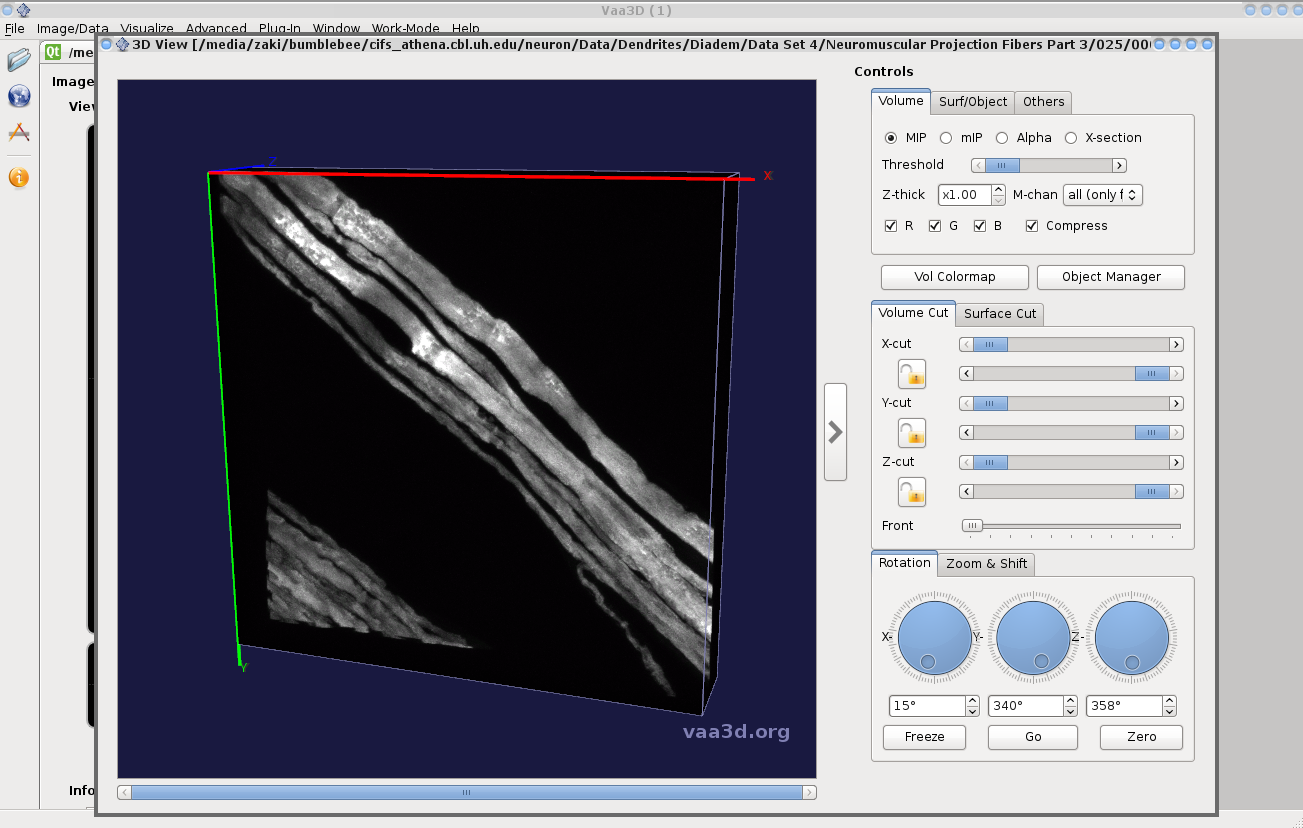
\includegraphics[width=0.8\textwidth]{gfx/vaa3d_DIADEM-NPF-3-025_3D-view}
\caption{Vaa3D: Visualization of NPF025 TIFF stack}
\end{figure}

\begin{figure}[H]
\centering
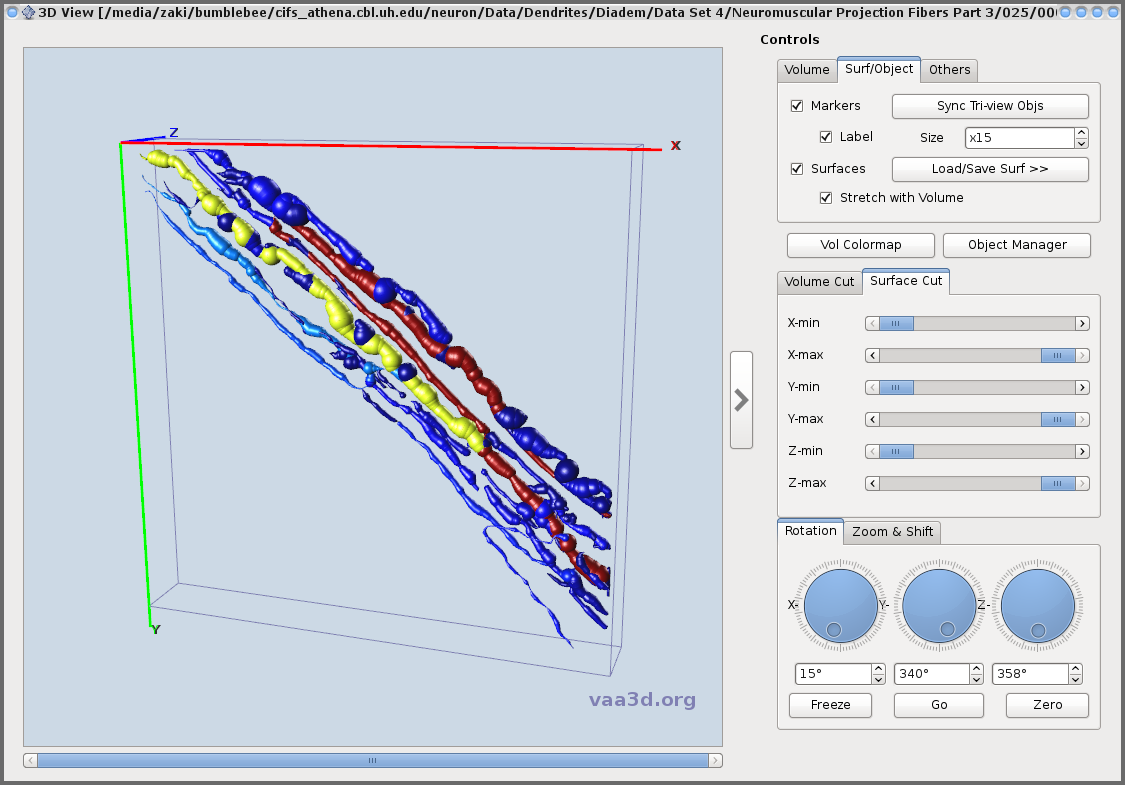
\includegraphics[width=0.8\textwidth]{gfx/vaa3d_DIADEM-NPF-3-025_APP2-tracing-3D-view}
\caption{Vaa3D: Tracing of NPF025 using Vaa3D APP2 plugin}
\end{figure}

\section{Testing and reproducibility}

\subsection{Input data}

\begin{itemize}
	\item Call graph of \gls{orionmat} (a digraph where each node is a
		function and each edge is a function call relationship where the first function
		node calls the second function node).
	\item Call graph of  \gls{orionc} with corresponding function nodes to
		those in the call graph of \gls{orionmat}.
	\item A sample of the volumes in NPF above.
\end{itemize}

\subsection{Procedure}

\begin{enumerate}
	\item Run the \gls{orionmat} code on a volume from the input data.
	\item For each call made in \gls{orionmat}, capture the
		parameters, return values, and output files of each function.
	\item For each node in the call graph of \gls{orionc}, pass the
		parameters of the corresponding \gls{orionmat} call and capture
		the return values from \gls{orionc} (note that there are no
		output files since \gls{orionc} works entirely in memory)
	\item Create a table that shows the difference in the results from each
		function call.
\end{enumerate}

\subsection{Results}

\begin{figure}
%\documentclass[tikz, border=10pt]{standalone}
\tikzset{
    vertex/.style = {
        circle,
        fill            = black,
        outer sep = 2pt,
        inner sep = 1pt,
    }
}

%\begin{document}

\newcommand{\myfun}[2] {$fun^{#1}_{#2}$}
  
\begin{tikzpicture}
  % Cases
  \definecolor{lgray}{RGB}{192,192,192}
  \definecolor{ngray}{RGB}{160,160,160}
  \definecolor{dgray}{RGB}{128,128,128}
  % Cases
  \definecolor{lblue}{RGB}{102,102,255}
  \definecolor{nblue}{RGB}{51,51,255}
  \definecolor{dblue}{RGB}{0,0,255}
% Input node
\node[draw,fill=black,text=white,rotate=90] (Input) at (2,2) {Input};  
  
% Matlab nodes
\node[draw,fill=lgray,text=white] (funM1) at ( 4,0) {\myfun{M}{1}};
\node[draw,fill=lgray,text=white] (funM2) at ( 7,0) {\myfun{M}{2}};
\node[draw,fill=lgray,text=white] (funM3) at (10,0) {\myfun{M}{3}};
\node[draw,fill=lgray,text=white] (funM4) at (13,0) {\myfun{M}{4}};
\node[draw,fill=lgray,text=white] (funM5) at (16,0) {\myfun{M}{5}};

% MC nodes
\node[draw,fill=ngray,text=white] (funMC1) at ( 4,2) {\myfun{M-C}{1}};
\node[draw,fill=ngray,text=white] (funMC2) at ( 7,2) {\myfun{M-C}{2}};
\node[draw,fill=ngray,text=white] (funMC3) at (10,2) {\myfun{M-C}{3}};
\node[draw,fill=ngray,text=white] (funMC4) at (13,2) {\myfun{M-C}{4}};
\node[draw,fill=ngray,text=white] (funMC5) at (16,2) {\myfun{M-C}{5}};

% C nodes
\node[draw,fill=dgray,text=white] (funC1) at ( 4,4) {\myfun{C}{1}};
\node[draw,fill=dgray,text=white] (funC2) at ( 7,4) {\myfun{C}{2}};
\node[draw,fill=dgray,text=white] (funC3) at (10,4) {\myfun{C}{3}};
\node[draw,fill=dgray,text=white] (funC4) at (13,4) {\myfun{C}{4}};
\node[draw,fill=dgray,text=white] (funC5) at (16,4) {\myfun{C}{5}};


% Initial data conection
\draw[->,draw=dblue] (Input) to[in=180,out=0] (funC1);
\draw[->,draw=nblue] (Input) to[in=180,out=0] (funMC1);
\draw[->,draw=lblue] (Input) to[in=180,out=0] (funM1);

% C
\draw[->,draw=dblue] (funC1) to[in=180,out=0] (funC2);
\draw[->,draw=dblue] (funC2) to[in=180,out=0] (funC3);
\draw[->,draw=dblue] (funC3) to[in=180,out=0] (funC4);
\draw[->,draw=dblue] (funC4) to[in=180,out=0] (funC5);

% MC
\draw[->,draw=nblue] (funM1) to[in=180,out=0] (funMC2);
\draw[->,draw=nblue] (funM2) to[in=180,out=0] (funMC3);
\draw[->,draw=nblue] (funM3) to[in=180,out=0] (funMC4);
\draw[->,draw=nblue] (funM4) to[in=180,out=0] (funMC5);

% M
\draw[->,draw=lblue] (funM1) to[in=180,out=0] (funM2);
\draw[->,draw=lblue] (funM2) to[in=180,out=0] (funM3);
\draw[->,draw=lblue] (funM3) to[in=180,out=0] (funM4);
\draw[->,draw=lblue] (funM4) to[in=180,out=0] (funM5);


\end{tikzpicture}

\begin{tikzpicture}
  % Dialectics
  \node[draw] (Thesis) at (0,0) {Thesis};
  \node[draw,fill=black,text=white] (Antithesis) at (2.3,0) {Antithesis};
  \node[draw,fill=gray,text=white] (Synthesis) at (1,2) {Synthesis};
  
  \draw node[vertex] (Joint) at (1,0) {};
  
  \draw[-,draw=blue] (Thesis) to (Joint);
  \draw[-,draw=blue] (Antithesis) to (Joint);
  \draw[->,draw=blue] (Joint) to (Synthesis);
  \draw[->,draw=blue] (Synthesis) to[in=180,out=180] (Thesis);
  
  \node at (1.0, -1.0) {\textit{a) Dialectics}};
  
  % Opposition
  \node[draw] (ArgumentA) at (5,0) {Argument};
  \node[draw,fill=black,text=white] (ArgumentB) at (7.5,0) {Opposition};
  
  \draw[->,draw=blue] (ArgumentA) to (ArgumentB);
  
  \node at (6., -1.0) {\textit{b) Opposition}};
  
  % Innovation
  \node[draw] (ArgumentA) at (10.1,0) {Argument};
  \node[draw,fill=black,text=white] (ArgumentB) at (13,0) {Opposition};
  \node[draw,fill=yellow] (ArgumentC) at (12,2) {Innovation};
  
  \draw node[vertex] (Joint) at (11.5,0) {};
  
  \draw[-] (ArgumentA) to (Joint);
  \draw[-] (ArgumentB) to (Joint);
  \draw[->,draw=blue] (Joint) to (ArgumentC);
  
  \node at (11.5, -1.0) {\textit{c) Innovation}};
\end{tikzpicture}
%\end{document}
\caption{Full pipeline}
\end{figure}

\end{document}
